\let\negmedspace\undefined
\let\negthickspace\undefined
\documentclass{article}
\usepackage{gvv-book}
\usepackage{gvv}
\usepackage{amsmath}
\usepackage{amsfonts}
\usepackage{tikz}
\usepackage{setspace}
\usepackage{gensymb}
\usepackage[cmex10]{amsmath}
\usepackage{amsthm}
\usepackage{mathrsfs}
\usepackage{txfonts}
\usepackage{stfloats}
\usepackage{bm}
\usepackage{cite}
\usepackage{cases}
\usepackage{subfig}
\usepackage{longtable}
\usepackage{multirow}
\usepackage{enumitem}
\usepackage{mathtools}
\usepackage{tikz}
\usepackage{circuitikz}
\usepackage{verbatim}
\usepackage[breaklinks=true]{hyperref}
\usepackage{tkz-euclide}
\usepackage{listings}
\usepackage{color}    
\usepackage{array}    
\usepackage{longtable}
\usepackage{calc}     
\usepackage{multirow} 
\usepackage{hhline}   
\usepackage{ifthen}   
\usepackage{lscape}     
\usepackage{chngcntr}
\usepackage{graphicx}
\usepackage{float}
\usepackage{multicol}
\usepackage[a4paper, left = 1.5cm, right = 1.5cm]{geometry}

%\newtheorem{theorem}{Theorem}[section]
%\newtheorem{theorem}{Theorem}[section]
%\newtheorem{problem}{Problem}
%\newtheorem{proposition}{Proposition}[section]
%\newtheorem{lemma}{Lemma}[section]
%\newtheorem{corollary}[theorem]{Corollary}
%\newtheorem{example}{Example}[section]
%\newtheorem{definition}[problem]{Definition}
\title{2.2.23}
\author{AI25BTECH110030 - SARVESH TAMGADE}
\begin{document}

{\let\newpage\relax\maketitle}

\textbf{Question}:

Find angle \(\theta\) between the vectors \(\vec{a} = \hat{i} + \hat{j} - \hat{k}\) and \(\vec{b} = \hat{i} - \hat{j} + \hat{k}\).

\vspace{2mm}
\textbf{Solution:}

Express vectors in column form:
\[
\vec{a} = \myvec{1 \\ 1 \\ -1},
\qquad
\vec{b} = \myvec{1 \\ -1 \\ 1}
\]

The cosine of the angle \(\theta\) is given by:
\[
\cos\theta = \frac{\vec{a}  \vec{b}}{\|\vec{a}\| \, \|\vec{b}\|}
\]

Compute dot product:
\[
\vec{a}  \vec{b} = (1)(1) + (1)(-1) + (-1)(1) = 1 - 1 - 1 = -1
\]

Compute magnitudes:
\[
\|\vec{a}\| = \sqrt{1^2 + 1^2 + (-1)^2} = \sqrt{3}
\]
\[
\|\vec{b}\| = \sqrt{1^2 + (-1)^2 + 1^2} = \sqrt{3}
\]

Substitute:
\[
\cos\theta = \frac{-1}{\sqrt{3}\sqrt{3}} = -\frac{1}{3}
\]
\[
\theta = \cos^{-1}\left(-\frac{1}{3}\right)
\]

\vspace{2mm}
\textbf{Answer:}

The required angle is:
\[
\boxed{\theta = \cos^{-1}\left(-\frac{1}{3}\right)}
\]



\textbf{Graph:}
\begin{figure}[H]
	\centering
	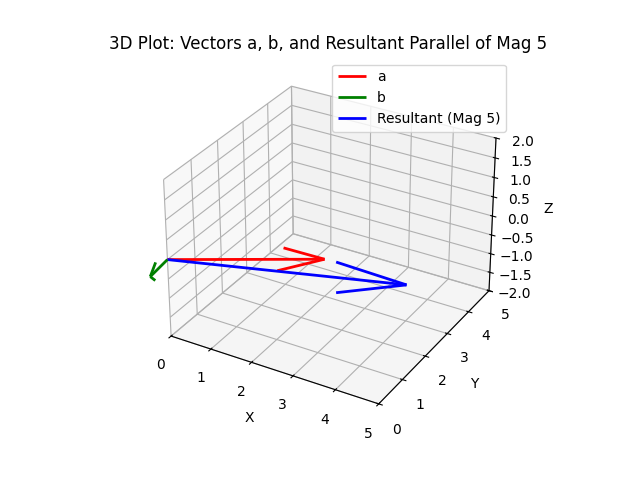
\includegraphics[width=0.8\columnwidth]{FIG/graph.png}
	\caption{3D Visualisation of two vectors and angle between them}
	\label{img}
\end{figure}
\end{document}
